%! Author = antoniomasotti
%! Date = 25.11.23

\subsection{Bob's story}
\begin{frame}{It all started with Bob...}
    \begin{center}
        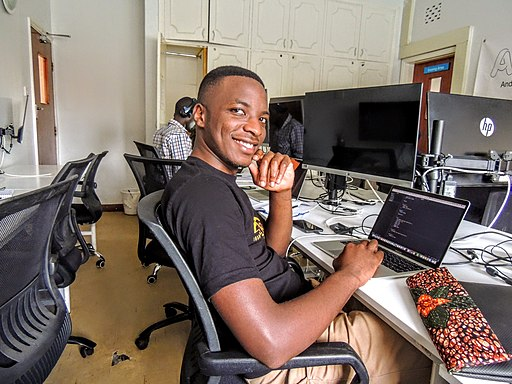
\includegraphics[width=.7\textwidth]{./assets/bob}

        \textbf{\Large{...and it continues with Bob}}
    \end{center}
\end{frame}

\begin{frame}
    \begin{center}
        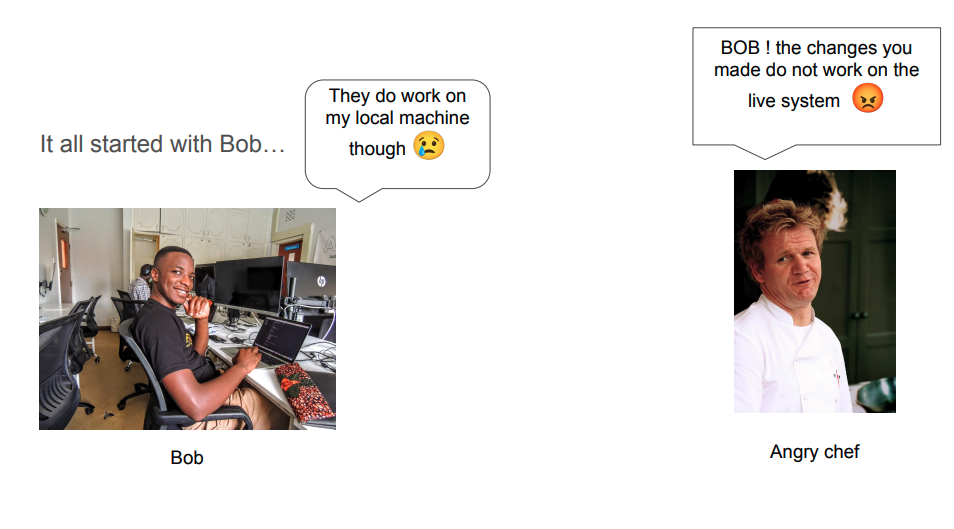
\includegraphics[width=.8\textwidth]{./assets/bob2}
    \end{center}
\end{frame}


\subsection{The wonderful world of microservices}
\begin{frame}{Bob has learnt the lesson...}
    \begin{center}
        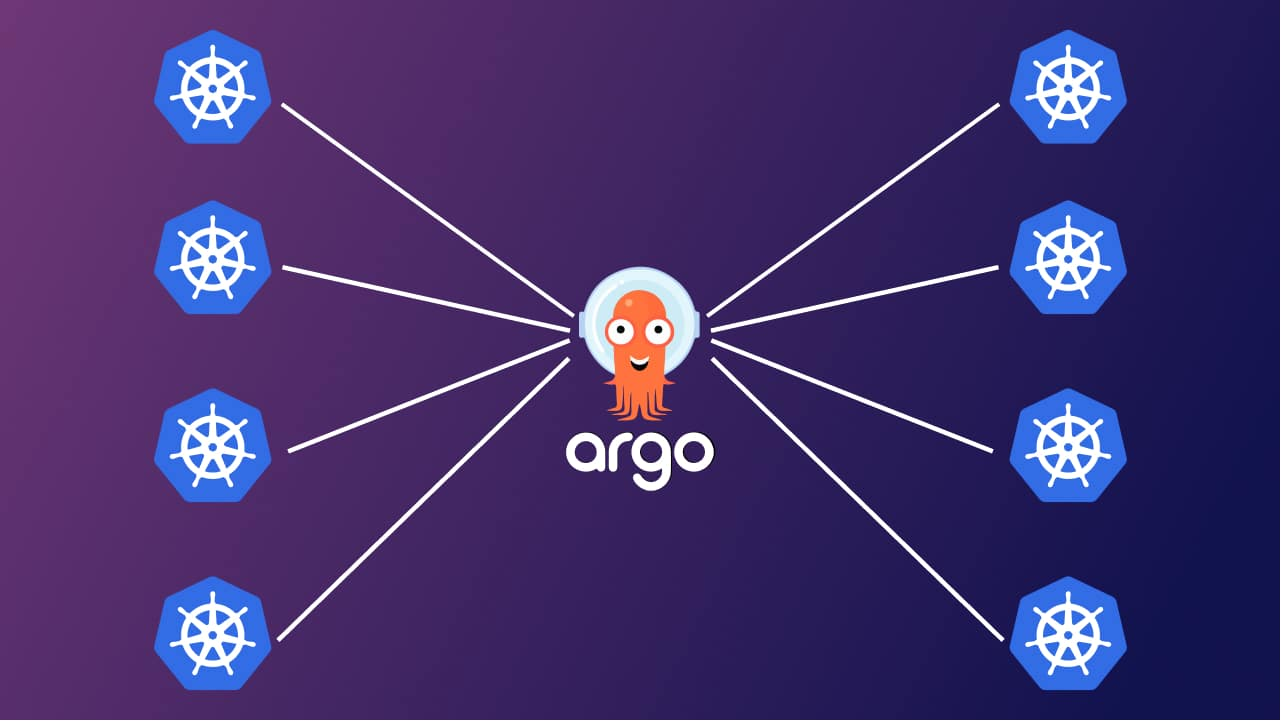
\includegraphics[width=.9\textwidth]{./assets/argocd}
    \end{center}
\end{frame}


\begin{frame}
    \begin{columns}
        \begin{column}{0.4\textwidth}
            \begin{center}
                
\includegraphics[width=.9\textwidth]{./assets/microservice_love}
            \end{center}
        \end{column}
        \begin{column}{0.6\textwidth}
            \begin{center}
                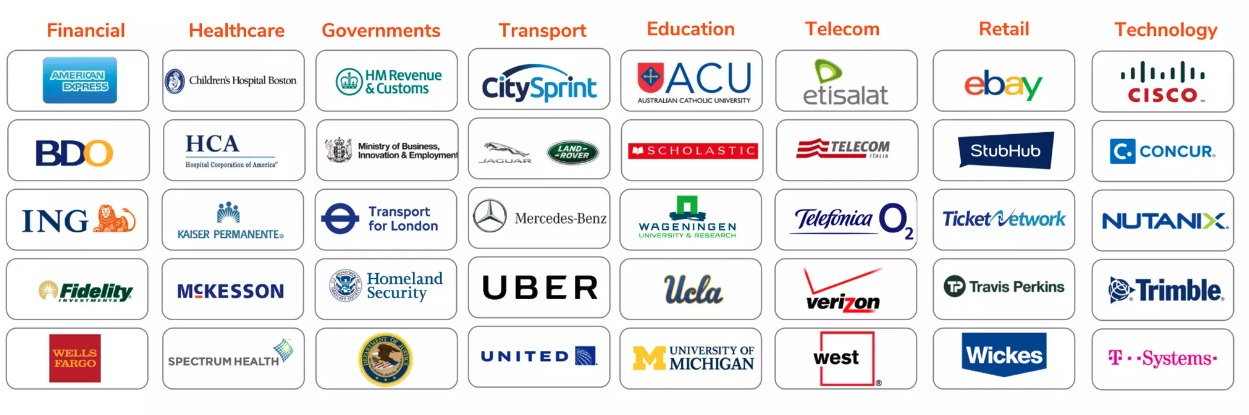
\includegraphics[width=1\textwidth]{./assets/microservices_companies}
            \end{center}
        \end{column}
    \end{columns}
\end{frame}

\begin{frame}{Extreme examples...}
    \begin{center}
        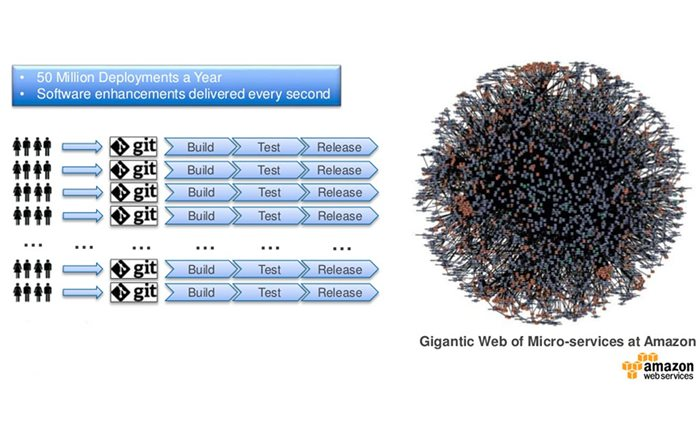
\includegraphics[width=.8\textwidth]{./assets/aws_microservices}
    \end{center}
\end{frame}

\begin{frame}{Benefits of microservices}
            \begin{itemize}[<+->]
            \item Big promise: Independent deployability
            \item Fast feedback loops
            \item Strong team focus, ideally crossfunctional
            \item Loosely coupled architecture
            \item Fast onboarding
            \item Cost-efficiency on the long run
            \item Cloud native
            \item Tech-agnostic approach
            \item Scalability out of the box
            \item Improved Security (no SPOF, no SPOC)
            \item Optimized Time to Market
            \end{itemize}
\end{frame}

\begin{frame}{Two key factors for success}
\begin{columns}
    \begin{column}{0.6\textwidth}
        \begin{shadequote}
            \small{
            \hspace{.5cm} Chief among the benefits of service-enabling an enterprise's
            application landscape are \textbf{increased organizational agility} and
            \textbf{reduced overall cost} of implementing change.

            \vspace{.3cm}

            A SOA increases organizational agility by placing high-value business functions
            in \textbf{discrete, reusable services}, and then connecting and orchestrating
            these services to satisfy core business processes.

            \vspace{.5cm}
            It reduces the cost of change by \textbf{reducing the dependencies} between services,
            allowing them \textbf{to be rapidly recomposed and tuned} in response to change or
            unplanned events.
            }
        \end{shadequote}
    \end{column}
    \begin{column}{0.4\textwidth}
        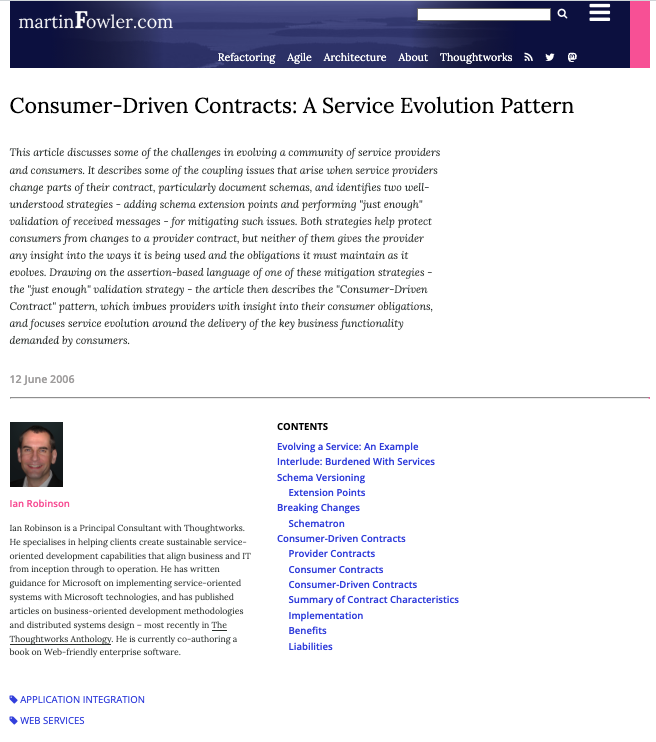
\includegraphics[width=1\textwidth]{./assets/ian_robinson}
    \end{column}
\end{columns}
\end{frame}

\begin{frame}
    \begin{center}
    \Huge{\textbf{But...}}
    \end{center}
\end{frame}


\begin{frame}{It's always a tradeoff}
\begin{columns}
    \begin{column}{0.6\textwidth}
        \begin{shadequote}
            \hspace{.5cm}
            The first (and probably only) law of software architecture states


            \textbf{“Everything in software architecture is a tradeoff”}

            \vspace{.3cm}

            -- Neal Ford
        \end{shadequote}
    \end{column}
    \begin{column}{0.4\textwidth}
        
\includegraphics[width=.8\textwidth]{./assets/software_architecture}
    \end{column}
\end{columns}
\end{frame}
